\documentclass[letterpaper,twocolumn,10pt]{article}
\usepackage{epsfig,endnotes}
\usepackage{times}
\usepackage{graphicx}
\usepackage{url}
\usepackage[usenames]{color}
\usepackage{indentfirst}
\usepackage{algorithm2e}

\setlength{\textwidth}{6.5in}
\setlength{\textheight}{9in}
\topmargin -0.75in
\columnsep 0.25in

\begin{document}
\title{\Large  C-Share: A Distributed File Sharing System Based on Chord Protocol}
\author{Boyu Zhang, Bo Song, Haoliang Zhang}

\date{}
\maketitle


\subsection*{Abstract}

The original chord paper introduces a decentralized peer-to-peer routing protocol using DHT (Distributed Hash Table). In terms of lookup efficiency, chord is scalable with the network size and can achieve an average O(log(n)) performance (where n denotes the number of nodes in the network). Using DHT to map node and data items onto a circular space, the leaving and joining of nodes will only require (with high probability) O(k/n) keys to be redistributed (where k denotes the total number of keys stored in the network).We built a file sharing system called C-Share that allows users to upload and download data files, and automatically deals with the placement of files when users leave or arrive. 

\section{Introduction}

Peer-to-peer communication protocol are widely used in distributed systems such as file sharing systems. The most important issue in building a distributed key storage system is the scalability and availability of data in a large-scale network. Traditional client-server model may suffer from master node failure, or very complex mechanisms in dealing with load balancing. One example of such system is the GFS (Google File System). It's designed to work in client-server model, where a master node is responsible for distributing data blocks onto each chunk server. The bottleneck of such a design lies in the master node because it may not have enough memory to hold all the metadata, and thus traffic through it must be carefully regulated. Also, it's claimed to be working in a relatively safe environment (inside Google) and node attacks are not prevalent.

Another design approach of a key storage system adopts the idea of decentralized paradigm. In such systems, every node has the same set of software library installed and is totally equal in functionality. In the vast literature of decentralized peer-to-peer communication protocols, we choose to build our file sharing system based on Chord because the protocol is simple and straightforward. It also has all the key features that fit in such a design category . In Chord, the routing information is evenly distributed to each chord node, every node in the network just needs to maintain a routing table (called the finger table) with much less memory footprint. It's able to locate a key in average logarithmic time by performing several hops between the nodes. Considering it to be applied in a dynamic environment where node joins and leaves are very common, Chord uses consistent hashing to guarantee minimum movement of keys during network changes. 

The rest of this report will be organized as follows: Section 2 will briefly talk about the related work in peer-to-peer communicating protocols. Section 3 will recap the core concepts in the original Chord paper. Section 4 will give a detailed discuss on our bidirectional search model. Section 5 will cover the details of implementation issues. Section 6 will give the experimental results. Section 7 will mainly discuss the lessons we've learned from this project. Section 8 will propose some directions of  future work. In section 9 we will come to a conclusion on this project.

\section{Related Work}

A typical P2P network is decentralized and treats all peers as equal participants. It allows the network to share contents to each other directly, and the failures of one node will not influence the functioning of other nodes, which makes the networks more reliable and does not have the bottleneck as the centralized network.

There are four distributed hash table protocols that are widely used in the P2P networks, including Chord, CAN, Pastry and Tapestry. Chord\cite{chord} is a distributed routing protocol, which maps from a key to a node in a structured P2P networks. It introduces a routing table called finger table to reduce the lookup in the network from O(N) to O(logN). Unlike Chord, both Pastry and Tapestry takes the node locality into consideration. Pastry\cite{pastry} is intended to perform application-level routing and object location in rather large overlay network environment and the expected routing steps are O(logN). But combined to Chord, Pastry is more complex while a node joining the network. Tapestry\cite{tapestry} is a self-organizing, scalable, robust wide-area infrastructure. Considering the network topology in Tapestry, messages will be routed to the closest copy of an object or services using only point-to-point links independently from location. However, Tapestry does not handle node arrivals and departures well. CAN\cite{CAN} (Content Addressable Network) is a distributed infrastructure which puts more emphasize on the scalability of the P2P system on Internet-like scales. With large increases in the number of nodes, the path length for routing increases slowly.

This project is based on Chord. Chord itself has the advantages of simplicity, provable correctness, and provable performance, but it also has some problems. Many further efforts have been made to address problems in Chord. PChord\cite{feng2006pchord} exploits the proximity of the underlying network topology, aiming to make up careless consideration of the routing locality in Chord. Similarly, TCS-Chord\cite{ye2005tcs} is also an improved topology-aware routing algorithm that clusters neighboring nodes and can perform better. Another paper\cite{chen2009improvement} improves Chord by removing redundant item information in the Finger Table and adding more information about nodes on the other half of the Chord ring, which cannot be reached by the original Chord model. It also considers the physical layer of the nodes to take advantage of the geography information. All these improvements result in promoting the efficiency of locating resources. S-Chord\cite{mesaros2002s} is one algorithm based on Chord, which can improve the lookup efficiency by 25\% for the worst-case. What differs S-Chord from Chord is that it maintains a symmetric routing table and also a symmetric routing policy.

\section{The original Chord protocol}

\subsection{Consistent Hashing}

The consistent hashing function assigns each node and key an $m$-bit identifier using a base hash function such as SHA-1. In the Chord network, each node's identifier is the hashcode of the node's IP address, and the data items are mapped to identifier keys by hashing its name. We will use node id for the identifier of node and key for the identifier of data item. Chord organizes all the node id and keys on a identifier circle modulo $2^{m}$. Key $k$ is assigned to the first node whose node id is equal to or follows $k$ in the identifier space. This node is called the successor node of key $k$, denoted by $successor(k)$. If identifiers are represented as a circle of numbers from 0 to $2^{m} - 1$, then $successor(k)$ is the first node clockwise from $k$.

Consistent hashing is designed to let nodes enter and leave the network with minimal disruption. When a node joins the network, only a small portion of its successor's keys are moved to it. When a node leaves the network, all of its responsible keys are moved to its successor. Under consistent hashing, the majority of keys are kept unmoved while only O(k/n) keys need to be reallocated, this induces very little system overhead in a dynamically changing network.

\subsection{Key Lookup in Chord}

To accelerate to key lookup process, every node maintains additional routing information. Let $m$ be the number of bits in the key/node identifiers. Every node maintains a finger table with at most $m$ entries. The $i^th$ entry in the table at node $n$ contains the identity of the first node $s$ that succeeds $n$ by at least $2^{i-1}$. According to the previous notation, $s = successor(n + 2^{i-1})$, and it's called the $i^th$ finger of node $n$.

This scheme has two important characteristics. First, every node knows more about nodes  closely following it on the identifier circle than about nodes farther away. Second, a node's finger table generally does not contain enough information to find the successor of an arbitrary key $k$. If node $n$ cannot decide the successor of key $k$, it will search through its finger table for a closest node $j$ that precedes $k$, and node $j$ is located more closer to the successor of $k$ and will know more about how to get there.

By repeating this process, $n$ can find the key's successor node in fairly small amount of hops. Theories have proven that the number of nodes to be contacted to find a successor in an $n$-node network is O(logn). This ensures the key lookup process with high scalability in case of large amounts of nodes are joined into the network.

\subsection{Nodes join and leave}

In a particular Chord network, nodes can join and leave at any time. The main challenge is preserving the the ability to locate every key in the network. When a node joins the network, it must initialize its own finger table and presumably, update other nodes' finger table to reflect this change. Each node in Chord maintains a predecessor pointer. It can be used to walk counterclockwise around the identifier circle.  The new node to be added learns the identity of an existing Chord node by some external mechanism (In our implementation, we use multicast to detect the existing chord node). Node $n$ learns its predecessor node by asking one of the existing node, and uses the predecessor's finger table as a starting point. After initialization, node $n$ needs to enter into the finger tables of some existing nodes. Node $n$ becomes the $i^th$ finger of node $p$ if $p$ precedes $n$ by at least $2^{i-1}$ and the $i^th$ finger of node $p$ succeeds $n$. For a given $n$, the algorithm starts with the $i^th$ finger of node $n$ and then continues to walk in the counter-clock-wise direction on the identifier circle until it encounters a node whose $i^th$ finger precede $n$. After node $n$ successfully initializes its own finger table and updates other nodes' finger table, it will contact its successor node for keys that it's responsible for, and add these keys to its own storage. In case of node leaving, node $n$ will do the reverse thing by contacting a series of nodes preceding it and asking them to delete the finger that points to it. Finally it moves all of the keys it stores locally to the successor node. This will need a little amount of network traffic to transfer the data items.

The original Chord paper didn't provide implementation for node leave. We provide our implementation as follows:

\begin{algorithm}
\eIf{n = successor()}{
return;\
}{
successor().predecessor = predecessor;\\
\While{i $\leq$ m}{
p = findPredecessor(n.id - $2^{i-1}$ + 1);\\
p.removeNode(n, i, successor());\\
i++;
} 
}
\caption{Node n leaving the Chord network}
\end{algorithm}

\begin{algorithm}
n.removeNode(n, i, repl)\\
\If{finger[i].node = n}{
finger[i].node = repl;\
predecessor.removeNode(n, i, repl);\
}
\caption{Remove node n}
\end{algorithm}

\section{Bidirectional key lookup process}

The motivation for proposing the bidirectional lookup is based on our observation that, in cases where the key's successor is located rightly preceding the current node on the chord ring, the original chord algorithm will always perform hops in a clockwise manner. It will traverse almost the whole Chord ring and perform much more hops(more RPC requests) than go in the counterclockwise direction.  The bidirectional link model is rather simple. In the model, a node needs to maintain a so-called reverse finger table in addition to the finger table. If there is a link in Chord, we will add a reverse link that links the same two nodes but at the reverse direction. For example, if node A is a finger of node B in Chord, i.e. there is a link from B to A, a reverse link from A to B will be added into the topology based on the bidirectional link model. Then, B becomes a reverse finger of A. There are no changes to the responsibility of data objects in Chord. All the data objects are still located at the successor nodes of their keys.

\subsection{Bidirectional lookup algorithm}

We take the finger table and the reverse finger table as a whole and call it the routing table. In the routing table, all the entries are ordered. To lookup a given key $k$, a node will check its routing table instead of only its finger table to find a certain table entry, namely one of its fingers or reverse fingers, whose identifier is closest to the key $k$ among all these entries. Then the lookup message is forwarded to the node referred by this entry. Finally, this lookup message will arrive at the node closest to the key $k$ among all the nodes in the network. Since we have not changed the responsibility of data objects, this node must be the predecessor or successor node of the key $k$. If the node is the successor node of $k$, the lookup is resolved. Or else, this node must be the predecessor node of $k$, the lookup is resolved too.

\begin{algorithm}
n.findSuccessor(k)\\
\eIf{k $\in$[predecessor.id, n.id]}{
return n;\
}{
\eIf{k $\in$[predecessor.id, n.id]}
{
return successor;\
}{
p = closestNode(k);\
return p.findSuccessor(k);\
}
}
\caption{ask node n to find successor of k}
\end{algorithm}

\begin{algorithm}
n.closestNode(k)\\
t=1;\\
x=finger[1];\\
\While{i $\leq$ $\mid$finger$\mid$}{
\If{$\mid$finger[i] - k$\mid$ $<$ $\mid$x - k$\mid$}{
x = finger[i];\\
t = i;\
}
i++;
}
return finger[t];
\caption{search for closest node to k}
\end{algorithm}

\section{System design and implementation}

\subsection{Design overview}

The objective of C-Share is to build a decentralized file sharing system for users to easily upload or download files without considering where the files are actually located. We provide C-Share as a user-space service that will take user's commands(such as 'save abc.cpp') and transform these commands to initiate an internal process that finally maps this file onto some node in the network. The C-Share running time will take care of maintaining finger table, initiate remote procedure calls, dispatching incoming requests, initiate a file transfer process, etc. The messaging subsystem serves as the core foundation of C-Share because all the inter-node communication, RPCs, file transfers are handled by this system. In the rest of this section, we will cover each part in greater detail.

\subsection{Messaging system}

In C-Share, the messaging system is responsible for remote function call and data transfer among different nodes. There are two categories of messages: RPC messages and Data messages. RPC messages are created when a node wants to call a function on a remote node and retrieve return value of that call. For example, if node i want node j to find the successor of key k, node i will call findSuccessor(k) on node j remotely. We use gRPC to implement this remote function call. Firstly, we need to write a .proto file to define the message type and structure as well as declare the protocol of remote function calls. Secondly, each node runs a gRPC server in a independent thread, listening to incoming calls. The server will extract parameters of the incoming calls, do some calculation, generate response and send it back to caller node. Finally, each node has a gRPC client class which defines all types of remote function call as its member functions. Back to our previous example, when node i want to call findSuccessor(k) on node j remotely, it will first connect to node j and get an object of gRPC client class. Then node j will call the member function findSuccessor(k) in this object and get the return value of it. In fact, the parameters and remote function name are all serialized and send to destination node via socket. The destination node deserializes it, demultiplexes it and calls the corresponding function calls with received parameters. Finally, the destination node retrieve the return value of the function call, serialize it and send it back to previously built socket. The source node deserializes the return value and the whole process is finished. All of these works are transparent to users and implemented by gRPC. 

\subsection{Chord message dispatcher}

As the chord network grows, each node will face with increasing amount of concurrent RPC requests. We implement a message dispatcher that can efficiently dispatch concurrent RPC requests to different working threads. Each dispatcher is bounded with a single chord node unit, and it will send out the requests to its corresponding chord node for execution. The dispatcher is responsible for accepting connections from other nodes, so it will have a single thread for listening. To reclaim the memory used by each finished working thread, the dispatcher also has a thread cleaner that runs in every 5 seconds to clean up all the finished threads. This also helps the system to keep a minimal memory footprint during execution.

\subsection{Chord node implementation}

The routing algorithm implementation are provided in the chordNode class. We define chordNode as a single entity that's responsible for maintaining the finger table, locating keys in a network, executing incoming chord messages, storing/retrieving files from the network, etc. 

Each chordNode maintains a pool of free chordMessagers, these messagers are used for processing concurrent requests. When the dispatcher receives a new request, it will pass the socket descriptor to one of the chordMessagers. When chordNode wants to initiate an RPC, it will claim a free chordMessager for this RPC transaction and establish a connection to the destination chordNode's dispatcher process. In general, RPC are handled in a consistent link between two chordMessagers of two different chordNodes. Once the RPC returns, the link will be closed and the two chordMessagers on the link's ends will be freed for handling future requests. In the situation when there are many concurrent connections between two nodes, this mechanism will provide much higher efficiency to allow for several messaging procedures to run at the same time.

The implementation of chordNode provides procedures introduced by the original chord paper. These procedures are essential for locating a key in the distributed chord network, including \textit{findSuccessor(key)},  \textit{findPredecessor(key)}, \textit{closestPrecedingFinger(key)}. In general, each procedure is paired with an RPC version of that procedure. These two types can be distinguished from the function parameters. The local version of procedure calls don't need pass in the node information as a parameter, whereas the RPC version of the procedure needs to pass in a parameter that specifies a remote node.  For example, the RPC version of \textit{findSuccessor(key)} looks like \textit{findRemoteSuccessor(node, key)}. A typical RPC transaction in C-Share works as follows (we assume node n initiates an RPC on node j):
\begin{enumerate}
	\item On node $n$, the RPC procedure creates a new message object, such as \textit{chordMessageFindSuccessor}, and the message object will contain all the parameters of the RPC.
	\item The RPC procedure will call \textit{makeRequest} by passing in the pointer to the message object.
	\item  \textit{makeRequest} will claim an available chordMessager, setting up the messager's remote hostname and port number to node $j$, and initiate it in the client mode. The chordMessager then tries to establish connection with the dispatcher process of node $j$.
	\item Node $j$'s dispatcher process receives the RPC message and creates a new thread to process this message.
	\item The newly initiated thread will claim an available chordMessager. Then it will deserialize the message and reconstructs the message object, pass its pointer to the chordNode's \textit{executeChordMessage} procedure.
	\item  The \textit{executeChordMessage} procedure will call the corresponding local procedure and create a new message object to store the return value of procedure.
	\item Node $j$'s processing thread will serialize the message object that stores return value, send it back to node n's chordMessager.
	\item On node n, the makeRequest procedure deserializes the incoming message and pass it back to the RPC procedure.

\end{enumerate}

\subsection{Existing node detection}
When a new node joins the chord network, it must find a way to get the information of some existing node to help initialize its finger table. The original chord paper doesn't talk much about this process. In our implementation, we used UDP multicast for detecting existing nodes. We assume that the chord nodes are located in the same IP group, such that every node in this group can receive the packets sent from any other node within that group.

The detection process in C-Share works as follows (we assume node $n$ joins):

\begin{enumerate}
	\item Node $n$ sends a multicast packet saying that 'I'm node n, I want to join now.'.
	\item  If after 5 trials, node $n$ hasn't received any feedback from other nodes, it regards itself as the first node in the network, go to 5. Otherwise go to 3.
	\item Node $n$ receives feedback packet from an existing node $j$, and node $j$ will attempt to connect with node $n$.
	\item Node $n$ and node $j$ are connected, and node $n$ can use node $j$'s finger table to initialize its own.
	\item Join completes.

\end{enumerate}

This mechanism works well in our testing environment, however, in some networks IP multicast or broadcast is abandoned. In these networks, we must use other external process to configure the existing node information.

\subsection{File transfer application}
The file transfer logic is easy to implement when we have built up all the messaging mechanisms and chord routing algorithms. C-Share provides users with 5 APIs related with file operation:

\noindent \textbf{storeFile} This API allows user to store a specific file to the chord network. It finds the location of the key and performs an addKey operation to the destination node. Then it sends the file data to the destination node's local disk storage.

\noindent\textbf{deleteFile} This API allows user to delete a file from the chord network. It first locates the key, then sends a removeKey and removeDataFile operation to the destination node.

\noindent \textbf{existFile} Use this API for checking the availability of a particular file. It simply checks whether the destination node contains this key and returns a boolean value.

\noindent \textbf{getFile} If the user wants to get a file that's stored on remote nodes, this API first check the existence of the file and then initiate a file transfer request to the destination node that holds the file.

\noindent \textbf{listFile} This API will return back all the keys that are currently stored in the chord network. It starts from the current node, traversing the identifier circle in clockwise using the successor pointer and collecting the keys stored on each node along the way.


\section{Experimental results}
To evaluate the performance of our C-Share system, we used average hops during key location as the major metric.  As discussed above, the key locating process may involve several hops to remote nodes. In our experiment, we use different processes to simulate each chord node. In our testing environment, it's very hard to use different machines to simulate a very large network, so we use different processes to stand for different nodes.  We run the C-share system and perform a series of random key lookup operations, and we get the following result.

We can see from the result(shown in Figure \ref{fig2}) that the number of hops is logarithmic to the number of nodes in the network, which means our system is scalable with network size.

\begin{figure}[!ht]
\centering
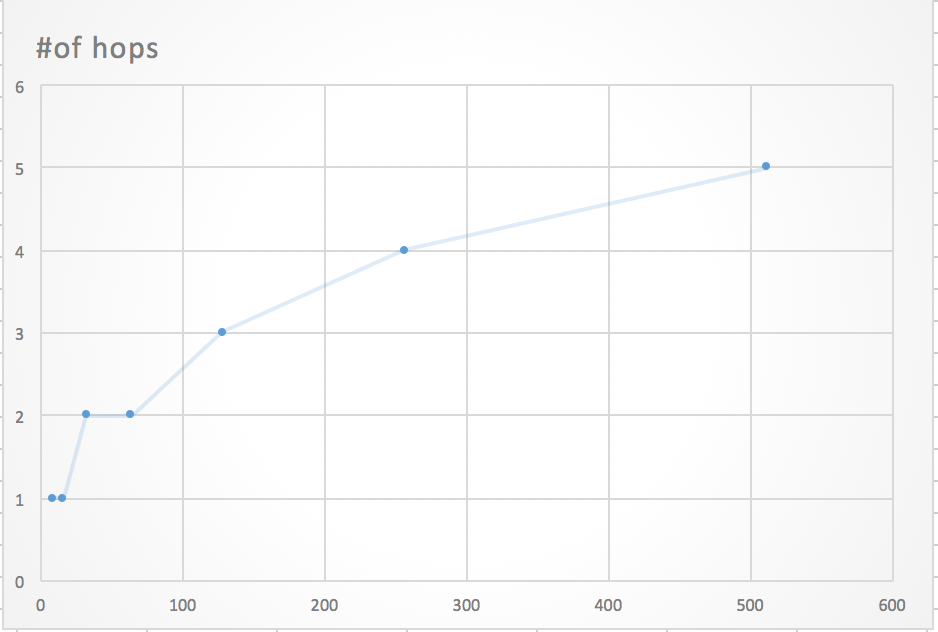
\includegraphics[width=60mm]{1.png}\\
\caption{Number of hops with network size increasing}
\label{fig2}
\end{figure}

\section{Lessons learned}
During the development of C-Share, we've experienced with a lot of challenging problems. We will discuss some of our experiences in this section.

\begin{enumerate}
	\item Simple design, clear abstraction

The architectural design of C-Share has taken lots of our effort. We find it very hard at the beginning to come up with a clear abstraction of software layers. During implementation, we overturned previous designs from time to time. Fortunately, the perspective of the project becomes much clearer as we implemented more modules. We think taking 30\% more time in achieving a good design will save us more than 30\% of time in the development process. Simple design also means easier to implement and debug.

\item Build a baseline system first

Any improvements of the original algorithm must be based on a stable realization of the basic algorithms. In the development process, we should also make the software modules easy to update to newer algorithms, rather than coupling many different parts together.

\end{enumerate}



\section{Future work}
Due to the project time limit, we haven't implemented all of the improvements. Some of our future work are:

\subsection{Bidirectional search}
Due to time limit, we haven't fully implemented the bidirectional search algorithm we present in this paper. However, the design of our system is flexible enough to employ a new search model, and we will implement this part in our future work.

\subsection{Hierarchical Chord ring}
Chord assumes that all nodes and data items are mapped on the single chord ring. As the network grows, the ring may become more crowded. If the nodes are located sparsely in several different network partitions, the key location process may become much slower. We can imagine a hierarchical ring that works like a ring of rings. Nodes within each network partition are placed in a virtual ring, and all these rings form a larger global virtual ring. This hierarchical layout of chord rings will improve key lookup considerably when nodes are distributed across heterogeneous network partitions. The first step in locating a key is to find the network partition this key resides in, and the second step is to confine the lookup process within that particular partition. This approach will minimize the messages exchanged between different partitions, making the key lookup process more efficient.

\section{Conclusions}
Using the Chord provides a distributed naming service for our peer-to-peer file sharing application. In our experiments, the Chord protocol has achieved the logarithmic key lookup performance as it's claimed in the original paper. During our development process, we have also fixed some bugs in the original Chord protocol(which will result in infinite RPCs in certain scenarios).





\bibliographystyle{acm}
\bibliography{template}

\end{document}
